Cette expérience permet d'observer l'impact du niveau de reconstruction des flux quand l'opérateur de diffusion est couplé à un opérateur de diffusion et faisant émerger des dynamiques de couplage.
L'équation de diffusion est donc remplacée par l'équation de Nagumo (voir \ref{par:analyser_operateurs_nagumo}).
Des ondes progressives sont solution de cette équation, le schéma numérique donc doit être en mesure de suivre la dynamique du front d'onde.

\subsubsection{Résumé de l'expérience}
L'expérience à été réalisée dans des conditions similaires à l'expérience numérique \ref{par:contrib_imex}. 
C'est à dire :
\begin{itemize}
    \item[$\diamond$] Profil de l'onde propagative comme état initial.
    \item[$\diamond$] Domaine étendu avec conditions de Neumann aux limites pour limiter les effets de bord
\end{itemize}
L'unique différence majeur est le remplacement de la méthode Runge et Kutta ImEx par un schéma de séparation d'opérateur avec une méthode stabilisée explicite pour la diffusion (ROCK 2 \cite{AbdulleMedovikov2001}).
Ce choix découle, comme précédemment expliqué, de la nécessité d'éviter toute inversion de système linéaire lorsque les flux sont reconstruits à partir de reconstructions
fines.
\subsubsection{Résultats de l'expérience}
Les résultats présentés à la figure \ref{fig:flux_reconstruction_nagumo} confirment les tendances observées sur la diffusion pure :

\begin{itemize}
    \item[$\diamond$] \textbf{Pas de temps élevés :} l'erreur est dominée par la discrétisation temporelle. Les trois approches (sans reconstruction, reconstruction partielle ou complète) montrent alors des précisions quasi identiques.
    \item[$\diamond$] \textbf{Pas de temps très faibles :} lorsque l'erreur spatiale devient prépondérante, la reconstruction fine des flux dégrade la solution. Plus les flux sont reconstruits, plus l'erreur augmente.
    \item[$\diamond$] \textbf{Influence des paramètres :} cette conclusion générale reste valable quels que soient les paramètres $k$ et $D$. Toutefois, lorsque la diffusion est prépondérante (valeurs de $D$ élevées), l'écart de précision entre la méthode sans reconstruction et celle avec reconstruction fine se creuse nettement.
    \item[$\diamond$] \textbf{Profils raides et pas intermédiaires :} pour des ondes très raides (réaction dominante), on observe à nouveau un effondrement brutal de l'erreur sur une gamme de pas de temps intermédiaires. Cet effet, déjà mis en évidence dans le cas ROCK2 sans reconstruction (voir~\ref{par:lien_rock_equiv}), semble lié à la géométrie du front d'onde et mériterait une investigation dédiée.
\end{itemize}
\newpage
\subsubsection{Conclusion de l'expérience sur Nagumo}
Cette série de simulations indique que l'ajout du terme de réaction dans l'équation de Nagumo ne modifie pas de façon radicale le couplage entre le schéma numérique et la MRA. 
Cela s'explique par le fait que la dégradation observée provient avant tout d'une prédiction des flux insuffisamment précise au regard de l'ordre spatial du schéma, 
indépendamment de la présence d'une réaction.
On note en outre que l'erreur introduite lors de la résolution du terme diffusif ne semble pas se propager au terme de réaction :
plus la diffusion domine (grand $D$), plus l'effet négatif de la reconstruction se renforce, ce qui suggère un découplage efficace assuré par le splitting de Strang.
Pour aller plus loin, une étude utilisant des méthodes ImEx partitionnées - qui coupleraient peut-être plus les erreurs - telles que PIROCK \cite{Abdulle2013}, appliquée à une équation de diffusion–réaction avec un terme réactif réellement raide
\footnote{On rappelle que la réaction dans l'équation de Nagumo n'est pas raide.}, serait pertinente afin de vérifier si ce comportement se maintient.
\begin{figure}[h!]
    \centering
    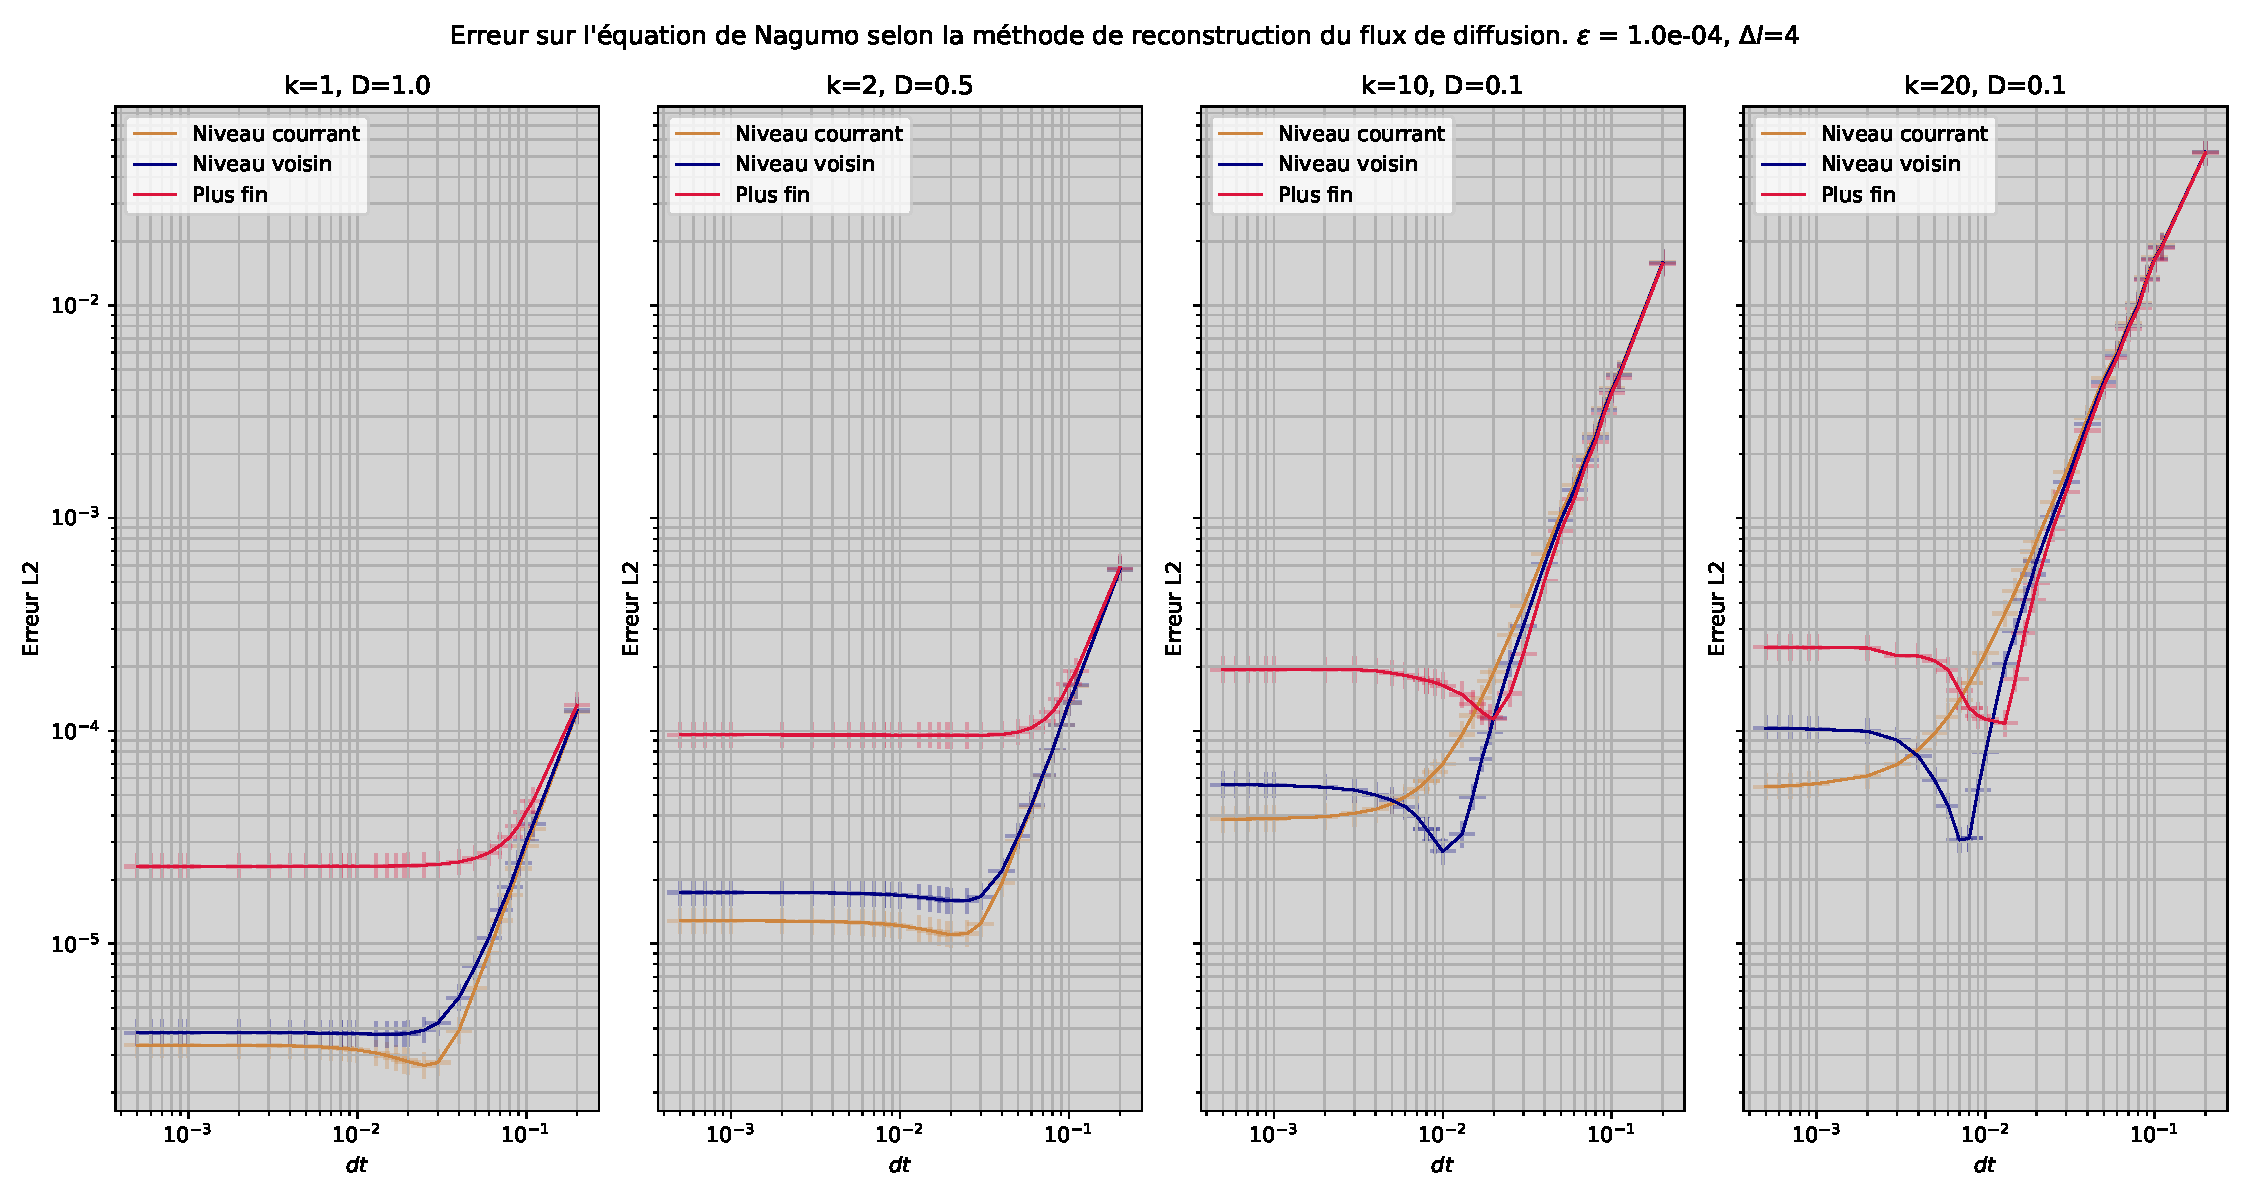
\includegraphics[width=\textwidth]{media/4_travail/3/flux_reconstruction_method_nagumo.pdf}
    \caption{Courbes de convergence de chaque méthode d'AMR pour différents paramètres de l'équation. Plus $k$ est élevé, plus le profil de l'onde est raide et plus la réaction domine. La célérité de l'onde est néanmoins identique pour chaque jeu de paramètres puisque le produit $kD$ reste constant d'une expérience à l'autre.}
    \label{fig:flux_reconstruction_nagumo}
\end{figure}